\documentclass[11pt,a4paper]{article}
\usepackage[T1]{fontenc}
\usepackage[utf8]{inputenc}
\usepackage[sc]{mathpazo}
\linespread{1.04}
\usepackage[scaled=0.86]{helvet}
\usepackage[margin=1in]{geometry}
\usepackage{amsmath,amssymb,amsthm,mathtools}
\usepackage{booktabs}
\usepackage{array}
\usepackage{tabularx}
\usepackage{float}
\usepackage[hidelinks]{hyperref}
\usepackage[nameinlink,noabbrev]{cleveref}
\usepackage{microtype}
\usepackage{enumitem}
\usepackage{siunitx}
\usepackage{xcolor}
\usepackage{caption}
\usepackage{tcolorbox}
\tcbuselibrary{skins,breakable}
\usepackage{thmtools}
\usepackage{tikz}
\usetikzlibrary{arrows.meta,positioning,calc,fit,backgrounds,matrix,decorations.pathmorphing}
\usepackage{pgfplots}
\pgfplotsset{compat=1.18}
\usepackage{longtable}
\usepackage{multirow}
\usepackage{makecell}
\usepackage{bm}
\usepackage{csquotes}
\usepackage{fancyhdr}
\usepackage{titlesec}

% ── Color palette ──
\definecolor{tfptblue}{RGB}{35,60,120}
\definecolor{tfptorange}{RGB}{190,100,20}
\definecolor{tfptgreen}{RGB}{40,110,60}
\definecolor{tfptgray}{RGB}{90,90,95}

\hypersetup{
    colorlinks=true,
    linkcolor=tfptblue!80!black,
    citecolor=tfptblue!70!black,
    urlcolor=tfptblue!60!black,
}

% ── Caption styling ──
\captionsetup{
    font={small,sf},
    labelfont={bf,color=tfptgray},
    labelsep=period,
    margin=1.5em,
    skip=6pt,
}

% ── Section heading styling ──
\titleformat{\section}
    {\Large\bfseries\color{tfptblue}}{\thesection}{0.8em}{}
\titleformat{\subsection}
    {\large\bfseries\color{tfptblue!85!black}}{\thesubsection}{0.7em}{}
\titleformat{\subsubsection}
    {\normalsize\bfseries\color{tfptblue!70!black}}{\thesubsubsection}{0.6em}{}
\titlespacing*{\section}{0pt}{1.8ex plus 0.6ex minus 0.3ex}{0.9ex plus 0.2ex}
\titlespacing*{\subsection}{0pt}{1.4ex plus 0.4ex minus 0.2ex}{0.6ex plus 0.1ex}

% ── Running headers ──
\pagestyle{fancy}
\setlength{\headheight}{22pt}
\fancyhf{}
\fancyhead[L]{\small\itshape\color{tfptgray} TFPT 4.5: Boundary Polarization and Closed-Branch Dynamics}
\fancyhead[R]{\small\color{tfptgray}\thepage}
\renewcommand{\headrulewidth}{0.4pt}
\renewcommand{\headrule}{\hbox to\headwidth{\color{tfptblue!30}\leaders\hrule height \headrulewidth\hfill}}
\fancypagestyle{plain}{\fancyhf{}\fancyfoot[C]{\small\color{tfptgray}\thepage}\renewcommand{\headrulewidth}{0pt}}

% ── tcolorbox global defaults ──
\tcbset{
    enhanced,
    boxrule=0.6pt,
    arc=2.5pt,
    left=6pt, right=6pt, top=5pt, bottom=5pt,
    fonttitle=\bfseries\sffamily\small,
    coltitle=white,
    toptitle=2pt, bottomtitle=2pt,
    shadow={0.8mm}{-0.6mm}{0mm}{black!12},
}

\sisetup{
    detect-all,
    round-mode = none,
    exponent-mode = input,
    exponent-product = \times,
    group-separator = {\,},
    group-minimum-digits = 4
}

\newtheorem{theorem}{Theorem}[section]
\newtheorem{corollary}[theorem]{Corollary}
\newtheorem{lemma}[theorem]{Lemma}
\theoremstyle{definition}
\newtheorem{definition}[theorem]{Definition}
\newtheorem{conjecture}[theorem]{Conjecture}
\newtheorem{proposition}[theorem]{Proposition}
\newtheorem{assumption}[theorem]{Assumption}
\newtheorem{axiom}[theorem]{Axiom}
\newtheorem{principle}[theorem]{Principle}
\newtheorem{construction}[theorem]{Construction}
\newtheorem{claim}[theorem]{Claim}
\newtheorem{appendixstep}[theorem]{Appendix Step}
\theoremstyle{remark}
\newtheorem*{remark}{Remark}

\crefformat{thmt@dummyctr}{Remark}
\Crefformat{thmt@dummyctr}{Remark}
\crefname{thmt@dummyctr}{remark}{remarks}
\Crefname{thmt@dummyctr}{Remark}{Remarks}
\crefname{conjecture}{conjecture}{conjectures}
\Crefname{conjecture}{Conjecture}{Conjectures}
\crefname{definition}{definition}{definitions}
\Crefname{definition}{Definition}{Definitions}

\makeatletter
\def\theHtheorem{\thesection.\thetheorem}
\def\theHcorollary{\theHtheorem}
\def\theHlemma{\theHtheorem}
\def\theHdefinition{\theHtheorem}
\def\theHconjecture{\theHtheorem}
\def\theHproposition{\theHtheorem}
\def\theHassumption{\theHtheorem}
\def\theHprinciple{\theHtheorem}
\def\theHconstruction{\theHtheorem}
\def\theHclaim{\theHtheorem}
\def\theHappendixstep{\theHtheorem}
\makeatother

\DeclareMathOperator{\tr}{Tr}
\DeclareMathOperator{\rank}{rank}
\DeclareMathOperator{\SF}{SF}
\DeclareMathOperator{\Ind}{Ind}
\DeclareMathOperator{\argmin}{arg\,min}

\newcolumntype{Y}{>{\raggedright\arraybackslash}X}

\newcommand{\Seam}{\Sigma}
\newcommand{\inv}{\iota}
\newcommand{\taudbl}{\tau_{\mathrm{dbl}}}
\newcommand{\iC}{\iota_{\mathrm C}}
\newcommand{\epscar}{\varepsilon_{\mathrm{car}}}
\newcommand{\Xbulk}{X_{\mathrm{bulk}}}
\newcommand{\Mpl}{\bar M_{\mathrm{Pl}}}
\newcommand{\Mplunred}{M_{\mathrm{Pl}}}
\newcommand{\cthree}{c_3}
\newcommand{\atheta}{a_\theta}
\newcommand{\phibase}{\varphi_{\mathrm{base}}}
\newcommand{\phiz}{\varphi_0^{\mathrm{ret}}}
\newcommand{\phiseam}{\varphi_{\Sigma}}
\newcommand{\deltatop}{\delta_{\mathrm{top}}}
\newcommand{\omegaCCEW}{\omega_{\mathrm{CC}}^{(2)}}
\newcommand{\bone}{b_1}
\newcommand{\SM}{\mathrm{SM}}
\newcommand{\QCD}{\mathrm{QCD}}
\newcommand{\Oadm}{\Omega_{\mathrm{adm}}}
\newcommand{\Cmin}{\mathcal C_{\min}}
\newcommand{\Ageom}{\mathcal A_{\mathrm{geom}}}
\newcommand{\Atrans}{\mathcal A_{\mathrm{trans}}}
\newcommand{\Arec}{\mathcal A_{\mathrm{rec}}}
\newcommand{\Aobs}{\mathcal A_{\mathrm{obs}}}
\newcommand{\Asing}{\mathcal A_{\mathrm{sing}}}
\newcommand{\Vadm}{\mathcal V_{\mathrm{adm}}}
\newcommand{\Hrel}{\mathcal H_{\mathrm{rel}}}
\newcommand{\Hhad}{\mathcal H_{\mathrm{had}}}
\newcommand{\Hhub}{H_{\mathrm{hub}}}
\newcommand{\Htot}{\mathcal H_{\mathrm{tot}}}
\newcommand{\Gammaeff}{\Gamma_{\mathrm{eff}}}
\newcommand{\lambdaY}{\lambda_Y}
\newcommand{\Pred}{\operatorname{Pred}}
\newcommand{\gcar}{g_{\mathrm{car}}}
\newcommand{\Hint}{\mathcal H_{\mathrm{int}}}
\newcommand{\Kadm}{K_{\mathrm{adm}}}
\newcommand{\Tmin}{\mathfrak T_{\mathrm{min}}}
\newcommand{\Tbound}{\mathfrak T_{\partial}^{\min}}
\newcommand{\Tprim}{\mathfrak T_{\mathrm{prim}}}
\newcommand{\chiseed}{\chi_{\mathrm{seed}}}
\newcommand{\chigeo}{\chi_{\mathrm{geo}}}
\newcommand{\chigeozero}{\chi_{\mathrm{geo},0}}
\newcommand{\APSdom}{\mathrm{APS}_{\mathrm{dom}}}
\newcommand{\APSfam}{\mathrm{APS}_{\mathrm{fam}}}
\newcommand{\vgeo}{v_{\mathrm{geo}}}
\newcommand{\vewref}{v_{\mathrm{EW}}^{\mathrm{ref}}}
\newcommand{\Dstart}{D_{\mathrm{start}}}
\newcommand{\Tcore}{\mathfrak T_{\mathrm{core}}}
\newcommand{\Tbridge}{\mathfrak T_{\mathrm{bridge}}}
\newcommand{\Tker}{\mathfrak T_{\mathrm{ker}}}
\newcommand{\Tcomp}{\mathfrak T_{\mathrm{comp}}}
\newcommand{\Padm}{P_{\mathrm{adm}}}
\newcommand{\Pprim}{P_{\mathrm{prim}}}
\newcommand{\Tpre}{\mathfrak T_{\mathrm{pre}}}
\newcommand{\Tstar}{\mathfrak T_{\star}}
\newcommand{\APSdomprov}{\mathrm{APS}_{\mathrm{dom}}^{\mathrm{prov}}}
\newcommand{\sigmaQCD}{\sigma_{\mathrm{QCD}}}
\newcommand{\Cseam}{\mathcal C_{\Sigma}}
\newcommand{\Ccyc}{\mathfrak C_{\Sigma}}
\newcommand{\Ffals}{\mathsf F_{\mathrm{fals}}}
\newcommand{\Rcmp}{\mathcal R_{\mathrm{cmp}}}
\newcommand{\wspin}{\varpi_{\mathrm{spin}}}
\newcommand{\PhysAdmOne}{\widehat{\mathrm{PhysAdm}}_1}
\newcommand{\ObsAdm}{\mathbf{Obs}_{\mathrm{adm}}}
\newcommand{\GrenTFPT}{\Gamma_{\mathrm{TFPT}}^{\mathrm{ren}}}
\newcommand{\OphysTFPT}{\mathbf O_{\mathrm{phys}}^{\mathrm{TFPT}}}
\newcommand{\OschemeTFPT}{\mathbf O_{\mathrm{scheme}}^{\mathrm{TFPT}}}
\newcommand{\SchGrp}{\mathbf{Sch}}
\newcommand{\Runiv}{\mathfrak R}
\newcommand{\Mop}{\mathfrak M}
\newcommand{\Mphys}{\mathfrak M_{\mathrm{phys}}}
\newcommand{\Mscheme}{\mathfrak M_{\mathrm{scheme}}}
\newcommand{\Rren}{\mathfrak R_{\mathrm{ren}}}
\newcommand{\Bind}{\mathcal B_{\mathrm{ind}}}
\newcommand{\Clrig}{\mathfrak{Cl}}
\newcommand{\Runivrig}{\overline{\Runiv}}
\newcommand{\Seedop}{\mathbf{Seed}^{\mathrm{op}}}
\newcommand{\Cseed}{\mathfrak C_{\mathrm{seed}}}
\newcommand{\triv}{\textup{triv}}
\newcommand{\rankess}{\rank_{\textup{ess}}}
\newcommand{\red}{\textup{red}}


% -- TFPT 4.5 split helpers --
\newcommand{\sourceDraft}{\texttt{../tfpt-42.tex}}
\newcommand{\paperstatus}{Draft split from \sourceDraft; theorem wording still inherits the status discipline of the source manuscript.}

\newenvironment{tfptfrontbox}
{\begin{tcolorbox}[colback=tfptblue!2, colframe=tfptblue!45, breakable,
    title={Scope box: inputs, contribution, non-claims, audit surface}, colbacktitle=tfptblue!65]}
{\end{tcolorbox}}

\newenvironment{tfptwarningbox}
{\begin{tcolorbox}[colback=tfptorange!4, colframe=tfptorange!55, breakable,
    title={Editorial guardrail}, colbacktitle=tfptorange!75]}
{\end{tcolorbox}}

\newenvironment{tfptsourcebox}
{\begin{tcolorbox}[colback=tfptgreen!3, colframe=tfptgreen!50, breakable,
    title={Source extraction map}, colbacktitle=tfptgreen!65]}
{\end{tcolorbox}}

\newcommand{\TFPTxref}[1]{\textup{[TFPT cross-reference: \texttt{\detokenize{#1}}]}}
\newcommand{\TFPTeqref}[1]{\textup{[TFPT equation: \texttt{\detokenize{#1}}]}}

\newenvironment{tfptclaimcontract}
{\begin{tcolorbox}[colback=tfptblue!2, colframe=tfptblue!50, breakable,
    title={Claim contract}, colbacktitle=tfptblue!70]\small}
{\end{tcolorbox}}

\newenvironment{tfptexports}
{\begin{tcolorbox}[colback=tfptgreen!3, colframe=tfptgreen!50, breakable,
    title={Exported objects}, colbacktitle=tfptgreen!65]}
{\end{tcolorbox}}



\title{\color{tfptblue}\textbf{Cosmology Interfaces of the TFPT Closed Branch}\\[0.35em]
{\Large Seam Transfer, Axion Sector, Reheating, and CMB Targets}}
\author{Stefan Hamann \and Alessandro Rizzo}
\date{{\normalsize\color{tfptgray}\sffamily Paper 6 of the TFPT 4.5 series -- \today}}

\begin{document}
\maketitle

\begin{abstract}
This paper isolates the downstream cosmology interface of TFPT. Cosmology is not used as a
primitive selector of the theory. It is read from the closed branch through seam transfer,
determinant-line phase, scalaron sector, axion interface, reheating input, leptogenesis input,
neutrino sector, CMB spectra, and conjectural sky-map realization targets.
\end{abstract}

\begin{tfptfrontbox}
\textbf{Inputs from previous papers.} Papers 1--5 supply the closed branch $\Tstar$, the carrier
packet, the precision branch, the admissible QFT sector, and the boundary-normalized metrology.

\textbf{New theorem contribution.} Downstream cosmology interfaces:
\[
\Lambda_{\mathrm{IR}}
=
\Mplunred^4\left[-\log\det_{\mathrm{adm}}(1-U_\Sigma)\right],
\qquad
S_\Sigma=\log\mu_\Sigma(\alpha_\star),
\qquad
N_{\mathrm{DW}}=1,
\]
with axion, reheating, leptogenesis, and CMB targets stated at their proper status levels.

\textbf{Not claimed here.} No carrier proofs, no full $\alpha$ derivation, no QFT closure proof,
and no Standard-Model packet proof.

\textbf{Falsification or audit surface.} The paper fails if CMB Stage 2 is sold as a theorem, if a
good CMB world is conflated with this observed sky realization, or if cosmology is allowed to tune
the primitive branch.
\end{tfptfrontbox}

\begin{tfptwarningbox}
CMB and E8 must never be written as hard theorem claims in this paper. Stage 1 is spectra. Stage 2
is sky realization as a conjectural or programmatic target.
\end{tfptwarningbox}


\begin{tfptclaimcontract}
\textbf{Claim.} Closed branch exports cosmology interface data: seam transfer, axion interface, reheating/leptogenesis inputs, and CMB Stage 1/2 targets.\par
\textbf{Inputs.} Fixed $\Tstar$, metrology layer, determinant-line phase, scalaron and neutrino sectors.\par
\textbf{First assumptions.} Infrared continuation and nonequilibrium solver are separate comparison-layer inputs.\par
\textbf{Proof status.} Downstream interface; Stage 2 sky realization is programmatic/conjectural.\par
\textbf{Kill condition.} Cosmology tunes the primitive branch or Stage 2 is presented as theorem-level sky reconstruction.\par
\end{tfptclaimcontract}

\tableofcontents

\section{Cosmology as Downstream Interface}

The closed branch is fixed before cosmology enters:
\[
\Tstar
\Rightarrow
(U_\Sigma,\det_{\mathrm{adm}},\text{scalaron branch},\text{neutrino sector})
\Rightarrow
\text{cosmology interfaces}.
\]
This section should make the nonprimitive status of cosmology explicit.

\section{Seam Transfer and Infrared Determinant}

The seam-transfer expression is
\[
\Lambda_{\mathrm{IR}}
=
\Mplunred^4\left[-\log\det_{\mathrm{adm}}(1-U_\Sigma)\right].
\]
The text should state which part is theorem-level interface data and which part is an empirical
comparison convention.

\section{Axion Interface}

The axion sector is recorded as
\[
S_\Sigma=\log\mu_\Sigma(\alpha_\star),
\qquad
N_{\mathrm{DW}}=1,
\qquad
\theta_i=\pi(1-\phiseam(\alpha_\star)).
\]
The axion interface belongs here because it depends on seam transfer and determinant-line phase,
not on the primitive carrier proof.

\section{Reheating, Leptogenesis, and Neutrino Inputs}

Reheating and leptogenesis are stated as downstream inputs supplied by the closed branch. The paper
should keep them status-coded and avoid turning the module into a hidden fit engine for later CMB
targets.

\section{CMB Stage 1: Spectra}

Stage 1 is the spectral target: transfer functions, angular spectra, and comparison rows. This
stage may define falsification targets and benchmark rows, but it does not claim a unique sky-map
realization.

\section{CMB Stage 2: Sky Realization}

Stage 2 is a conjectural realization target. The source draft's distinction should remain explicit:
a good CMB world is not automatically this CMB world. The map-realization layer therefore belongs
in a programmatic or conditional section, not in the theorem stack.

\section{Downstream Obligations Moved to the Companion}

\begin{center}
\begin{tabularx}{\textwidth}{@{}p{0.28\textwidth}Y@{}}
\toprule
\textbf{Module} & \textbf{Status in this paper} \\
\midrule
Stationary horizons and compact objects & Listed only as downstream programmatic obligations; technical material is in the Companion. \\
Code subspace, pointer dynamics, and record algebra & Not part of the cosmology-interface proof surface. \\
Transient event channels & Falsification and prediction semantics belong to the Companion. \\
Pole masses, Higgs readout, and full flavor output & Inputs from earlier readout papers or Companion ledgers, not cosmology claims. \\
Extended comparison ledgers & Companion-only material. \\
\bottomrule
\end{tabularx}
\end{center}

\clearpage
\section{Main Technical Development}

This section contains the main technical development assigned to this paper by the TFPT 4.5 clean split. Cross-paper background is referenced through dependency and scope boxes; extended backend material is kept in the Technical Companion.

% Auto-extracted from ../tfpt-42.tex for the TFPT 4.5 clean split.
% Source body assigned by the TFPT 4.5 clean split.

% ---- FRW reduction, seam transfer, scalaron branch, falsification matrix, and proof-obligation ledger: source lines 9747-10259 ----
\section{FRW reduction, seam transfer, and the scalaron branch}
\label{sec:cosmology-closure}

The trace-class seam transfer belongs to the main reconstruction surface. The cosmological
constant and the reduced scalaron / determinant-line dynamics are therefore fixed directly on the
closed branch. Axion, reheating, and leptogenesis quantities are read through explicit interface
formulas built from the same theorem-level objects $U_\Sigma$, $a_\Sigma$, and the positive
scalaron sector $\mathcal H_{\mathrm{sc}}$.

\begin{theorem}[Trace-class seam transfer]
\label{lem:automatic-seam-transfer-convergence}
On the closed branch the seam transfer operator
\[
U_\Sigma:=\Padm e^{-\ell_\Seam|B_\Seam|}\Padm
\]
is positive and trace class. Hence
\[
0<\rho(U_\Sigma)<1,
\qquad
0<U_\Sigma<\Padm.
\]
so the Fredholm determinant
\[
-\log\det_{\mathrm{adm}}(1-U_\Sigma)
\]
converges absolutely and defines a positive quantity.
\end{theorem}

\begin{proposition}[Seam damping readout from electromagnetic closure]
\label{prop:seam-action-cosmology}
Let $\alpha_\star$ be the unique electromagnetic fixed point of
\TFPTxref{thm:alpha-canonical}. Define the closed seam damping by
\[
S_\Sigma:=-\log\rho(U_\Sigma).
\]
Then
\[
S_\Sigma
=
\log\mu_\Sigma(\alpha_\star)
=
\log\!\bigl(\phiseam(\alpha_\star)^{-1}\bigr)
=
\frac{\alpha_\star^2(\alpha_\star-2\cthree^3)}{8\cthree^6\,b_1}.
\]
\end{proposition}

\begin{proof}
At the electromagnetic fixed point, \TFPTxref{eq:carrier-cfe} is equivalent to
\[
\log\mu_\Sigma(\alpha_\star)
=
\frac{\alpha_\star^2(\alpha_\star-2\cthree^3)}{8\cthree^6\,b_1}.
\]
The seam transfer operator
\[
U_\Sigma=\Padm e^{-\ell_\Seam|B_\Seam|}\Padm
\]
uses the same admissible determinant sector as the electromagnetic closure. Its spectral radius
therefore defines the same exponential damping scale, so
\[
S_\Sigma
=
\log\mu_\Sigma(\alpha_\star)
=
\log\!\bigl(\phiseam(\alpha_\star)^{-1}\bigr).
\]
\end{proof}

\begin{theorem}[Infrared cosmological constant from seam transfer]
\label{thm:cosmology-closure}
\[
U_\Sigma:=\Padm e^{-\ell_\Seam |B_\Seam|}\Padm,
\qquad
S_\Sigma:=-\log\rho(U_\Sigma)=\log\mu_\Sigma(\alpha_\star),
\]
Then
\[
\Lambda_{\mathrm{IR}}
=
\Mplunred^4
\Bigl[-\log\det\nolimits_{\mathrm{adm}}(1-U_\Sigma)\Bigr]
\]
is well defined and positive on the closed branch, and
\[
0<U_\Sigma\le e^{-S_\Sigma}\Padm<\Padm.
\]
\end{theorem}

\begin{proof}
\Cref{lem:automatic-seam-transfer-convergence} gives trace-class positivity of
$U_\Sigma$, while \Cref{prop:seam-action-cosmology} fixes the intrinsic seam damping $S_\Sigma$.
Hence the determinant is well defined and positive, and so is the induced cosmological constant.
\end{proof}

\begin{corollary}[Determinant bounds for the infrared seam transfer]
\label{cor:ir-seam-transfer-bounds}
Let $\{\lambda_j(U_\Sigma)\}$ denote the admissible eigenvalues of the positive trace-class
operator $U_\Sigma$. Then
\[
\tr_{\mathrm{adm}}U_\Sigma
\le
-\log\det\nolimits_{\mathrm{adm}}(1-U_\Sigma)
\le
\frac{-\log(1-\rho(U_\Sigma))}{\rho(U_\Sigma)}\,\tr_{\mathrm{adm}}U_\Sigma.
\]
If, moreover, the infrared seam transfer is rank one,
\[
U_\Sigma=\rho(U_\Sigma)\,P_\Sigma^{(1)},
\]
then
\[
\frac{\Lambda_{\mathrm{IR}}}{\Mplunred^4}
=
-\log(1-\rho(U_\Sigma))
=
\rho(U_\Sigma)+O\!\bigl(\rho(U_\Sigma)^2\bigr).
\]
\end{corollary}

\begin{proof}
Because $U_\Sigma$ is positive trace class, its eigenvalues satisfy
\[
0<\lambda_j(U_\Sigma)\le \rho(U_\Sigma)<1.
\]
For every $x\in[0,\rho(U_\Sigma)]$ one has the scalar bounds
\[
x\le -\log(1-x)\le \frac{-\log(1-\rho(U_\Sigma))}{\rho(U_\Sigma)}\,x.
\]
Applying this to each eigenvalue and summing gives the determinant bounds. If
$U_\Sigma=\rho(U_\Sigma)P_\Sigma^{(1)}$ is rank one, then
\[
\det\nolimits_{\mathrm{adm}}(1-U_\Sigma)=1-\rho(U_\Sigma),
\]
and the Taylor expansion of $-\log(1-\rho)$ yields the displayed asymptotic formula.
\end{proof}

\begin{remark}[Status of numerical infrared readouts]
The theorem-level content of the present section is the determinant formula of
\TFPTxref{thm:cosmology-closure} together with the spectral bounds of
\TFPTxref{cor:ir-seam-transfer-bounds}. Any specific
\[
\frac{\Lambda_{\mathrm{IR}}}{\Mplunred^4}\sim 10^{-123}
\]
evaluation requires an additional infrared continuation and is therefore kept in
Appendix~\ref{app:ir-seam-continuations}.
\end{remark}

\begin{theorem}[\textnormal{[A]} Determinant-line axion interface and scalaron reheating data]
\label{thm:axion-seam-phase}
The closed branch contains the unique compact determinant-line phase
\[
a_\Sigma\in S^1_{\det}.
\]
By \TFPTxref{thm:boundary-winding-control}, the canonical branch has
\[
N_{\mathrm{DW}}=1,
\]
and the closed-branch initial displacement is
\[
\theta_i:=\pi\bigl(1-\phiseam(\alpha_\star)\bigr).
\]
The axion-interface formula is
\[
\Omega_a h^2=
\Delta_R^{-1}
\bigl[
\Omega_a^{\mathrm{mis}}(f_a,m_a,\theta_i)
+
\Omega_a^{\mathrm{str}}(f_a,N_{\mathrm{DW}})
\bigr].
\]
The scalaron reheating input is
\[
T_R=
\left(\frac{90}{\pi^2 g_\ast}\right)^{1/4}
\sqrt{\Gamma_\varphi \Mplunred}.
\]
These formulas define closed-branch interface data. Numerical late-time abundance and baryogenesis
readouts are obtained only after the declared cosmology comparison layer has fixed the relevant
infrared continuation and nonequilibrium solver.
\end{theorem}

\begin{proof}
The determinant-line phase theorem fixes the compact branch variable $a_\Sigma$, and
\TFPTxref{thm:boundary-winding-control} fixes the domain-wall number $N_{\mathrm{DW}}=1$ on the
canonical branch. The electromagnetic closure fixes $\alpha_\star$ and therefore the initial
displacement $\theta_i=\pi(1-\phiseam(\alpha_\star))$. Substituting these branch data into the
standard misalignment-plus-string formula gives the displayed axion-interface expression. The
scalaron reheating input is fixed by the $R^2$ branch through the displayed decay-width formula.
The numerical late-time readouts depend on additional infrared and nonequilibrium choices and are
therefore comparison-layer outputs rather than closed theorem-level numbers.
\end{proof}

\begin{theorem}[Boundary winding controls family, transport, and determinant closure]
\label{thm:boundary-winding-control}
Let
\[
n:=\SF(B_\Sigma)
\]
denote the spectral winding number of the boundary class on the admissible branch. Then
\[
N_{\mathrm{fam}}=3n,
\qquad
N_{\mathrm{DW}}=n,
\qquad
\sum_{f,j}L_{f,j}=40n.
\]
In particular the canonical rigid branch has $n=1$, hence $N_{\mathrm{fam}}=3$ and
$N_{\mathrm{DW}}=1$.
\end{theorem}

\begin{proof}
By \TFPTxref{thm:primitive-seam-generator}, the primitive branch carries the positive generator
$[u_\Sigma]=1$ and therefore one unit of seam spectral flow:
\[
n:=\SF(U_\Sigma)=1.
\]
The three displayed quantities scale linearly with seam winding on the retained branch.

First, each full winding repeats the quarter-turn corner balance once, and the family theorem
assigns three family units to one such primitive winding. Hence
\[
N_{\mathrm{fam}}=3n.
\]

Second, the determinant-line phase winds once per primitive seam winding, so the domain-wall number
tracks the same winding:
\[
N_{\mathrm{DW}}=n.
\]

Third, the transport excess is locked by the exact word-length sum rule, and one primitive winding
carries the canonical value $40$. Repeating the same winding $n$ times replicates the same closed
transport sector $n$ times, so
\[
\sum_{f,j}L_{f,j}=40n.
\]

Substituting $n=1$ gives
\[
N_{\mathrm{fam}}=3,
\qquad
N_{\mathrm{DW}}=1,
\qquad
\sum_{f,j}L_{f,j}=40.
\]
No appeal to the later canonical uniqueness theorem is needed.
\end{proof}

\begin{theorem}[\textnormal{[A]} Canonical leptogenesis interface on the closed branch]
\label{thm:leptogenesis-closure}
The closed branch fixes the heavy-neutrino spectrum, the family frame, and the reheating scale
entering flavored leptogenesis. The numerical baryon asymmetry is obtained only after solving the
corresponding Boltzmann system, which is treated as a comparison layer in the present manuscript.
\end{theorem}

\begin{proof}
\TFPTxref{thm:neutrino-closure} fixes the heavy/light neutrino data on the same admissible branch, so
the masses entering the flavored decay asymmetries are branch invariants. The hard holonomy closure
fixes the family frame, so the CP asymmetries and washout data are determined up to the same
closed-branch input package. On the reheating side, \Cref{thm:axion-seam-phase} fixes the
reheating-scale input $T_R$. These data are the theorem-level inputs to the flavored Boltzmann
system. The numerical asymmetry itself is then a solution of that system rather than a closed
main-text theorem of the core manuscript.
\end{proof}

\begin{theorem}[\textnormal{[A]} FRW reduction and cosmology interface data on the closed branch]
\label{thm:frw-cosmology-derivation}
Restrict the same closed-branch action to homogeneous and isotropic variables
\[
(a(t),\varphi(t),\theta_\Sigma(t),N_i(t)).
\]
Then the reduced action takes the form
\[
\begin{aligned}
S_{\mathrm{FRW}}
=
\int dt\,a^3\Big[
-3\Mpl^2\Hhub^2
+\frac12\dot\varphi^2
-V_{\mathrm{sc}}(\varphi)
\\
&\qquad
+\frac12 f_a^2\dot\theta_\Sigma^2
\\
&\qquad
-\chi_{\mathrm{top}}(\varphi)\bigl(1-\cos(N_{\mathrm{DW}}\theta_\Sigma)\bigr)
\Big]
\\
&\qquad
+S_{\mathrm{RH}}+S_{\mathrm{LG}},
\end{aligned}
\]
with
\[
\Lambda_{\mathrm{IR}}
=
\Mplunred^4\bigl[-\log\det\nolimits_{\mathrm{adm}}(1-U_\Sigma)\bigr],
\qquad
N_{\mathrm{DW}}=1,
\qquad
\theta_i=\pi\bigl(1-\phiseam(\alpha_\star)\bigr).
\]
The reduced action therefore fixes the low-curvature scalaron FRW sector and the closed-branch
cosmology interface data
\[
(\Lambda_{\mathrm{IR}},N_{\mathrm{DW}},\theta_i,T_R,\mathcal I_{\mathrm{LG}}),
\]
where $\mathcal I_{\mathrm{LG}}$ denotes the reheating / leptogenesis input block. Numerical axion
abundance and baryon-asymmetry readouts are obtained only after solving the corresponding
nonequilibrium system in the comparison layer.
\end{theorem}

\begin{proof}
\Cref{thm:full-frw-interface-theorem} supplies the manuscript-level proof of the reduced FRW action
and of the closed-branch interface tuple
\[
(\Lambda_{\mathrm{IR}},N_{\mathrm{DW}},\theta_i,T_R,\mathcal I_{\mathrm{LG}}).
\]
Its ingredients are exactly the geometric Hodge branch, the seam-transfer determinant, the
determinant-line axion reduction, and the leptogenesis interface data already fixed in the main
text. Therefore the FRW reduction and the resulting cosmology interface package are theorem-level
outputs of the same closed branch, while the final late-time abundance and baryogenesis numbers
remain in the comparison layer.
\end{proof}

\begin{corollary}[No extra dark WIMP sector required]
The minimal closed branch has dominant axionlike dark matter and the only
irreducible hot dark component is the neutrino background. No extra dark WIMP sector is required
for closure.
\end{corollary}

The theorem-level output branching is summarized in \Cref{fig:cosmology-output-flow}.

\begin{figure}[t]
\centering
\scriptsize
\begin{tikzpicture}[
    >=Latex,
    source/.style={draw=blue!60!black, fill=blue!6, rounded corners, text width=2.55cm, minimum height=0.95cm, align=center},
    mid/.style={draw=orange!75!black, fill=orange!8, rounded corners, text width=2.55cm, minimum height=0.95cm, align=center},
    result/.style={draw=green!50!black, fill=green!8, rounded corners, text width=2.55cm, minimum height=0.95cm, align=center}
]
\node[source] (useam) at (-4.8,1.45) {$U_\Sigma$\\trace-class seam transfer};
\node[source] (alpha) at (-1.6,1.45) {$\alpha_\star,\ \phiseam(\alpha_\star)$\\electromagnetic closure};
\node[source] (asig)  at (1.6,1.45) {$a_\Sigma$\\compact determinant phase};
\node[source] (neut)  at (4.8,1.45) {family / neutrino sector\\closed branch data};

\node[mid] (ssig) at (-4.8,-0.25) {$S_\Sigma=-\log\rho(U_\Sigma)$\\intrinsic seam damping};
\node[mid] (thetai) at (-1.6,-0.25) {$\theta_i=\pi(1-\phiseam(\alpha_\star))$\\initial displacement};
\node[mid] (ndw) at (1.6,-0.25) {$N_{\mathrm{DW}}=1$\\from boundary winding};
\node[mid] (scal) at (4.8,-0.25) {$R^2$ / scalaron branch\\reheating channel};

\node[result] (lambda) at (-4.8,-2.15) {$\Lambda_{\mathrm{IR}}$\\positive seam-transfer output};
\node[result] (omegaa) at (0,-2.15) {$\Omega_a h^2$\\axion interface};
\node[result] (tr) at (3.2,-2.15) {$T_R$\\reheating input};
\node[result] (eta) at (6.4,-2.15) {$\mathcal I_{\mathrm{LG}}$\\Boltzmann input map};

\draw[->, thick] (useam) -- (ssig);
\draw[->, thick] (ssig) -- (lambda);
\draw[->, thick] (alpha) -- (thetai);
\draw[->, thick] (asig) -- (ndw);
\draw[->, thick] (thetai) -- (omegaa);
\draw[->, thick] (ndw) -- (omegaa);
\draw[->, thick] (scal) -- (tr);
\draw[->, thick] (neut) -- (eta);
\end{tikzpicture}
\caption{Cosmology interface data on the closed branch. Seam transfer, determinant-line phase, and
the scalaron / neutrino sectors generate $\Lambda_{\mathrm{IR}}$ together with the axion,
reheating, and leptogenesis input block; final late-time numerical readouts are comparison-layer
outputs.}
\label{fig:cosmology-output-flow}
\end{figure}

\begin{remark}[Closed-branch reading]
These cosmological quantities are derived on the closed branch from the same retained operator
data. They are no longer ad hoc bridge readouts, but they are also not all final theorem-level
numbers: the main text fixes the cosmology interface data, while late-time abundance and
leptogenesis numerics remain comparison-layer outputs.
\end{remark}

Appendix-level E$_8$ arithmetic continuations and asymptotic scale-grammar formulas are collected
in Appendix~\TFPTxref{app:constants} and are not part of the main theorem surface.

\subsection{Falsification matrix}

The present draft does not ask the reader to accept one undifferentiated output claim. Each
main-text closure statement has a corresponding local or global failure mode, and those failure
modes should be readable without first decoding the appendix tables.

The matrix below is therefore intentionally short. It collects only the load-bearing main-paper statements whose failure would break the boundary-polarized architecture at the theorem level, rather than every downstream benchmark row or optional appendix interface.

\begin{table}[t]
\centering
\small
\begin{tabularx}{\linewidth}{@{}>{\raggedright\arraybackslash}p{0.24\linewidth}YY>{\raggedright\arraybackslash}p{0.13\linewidth}@{}}
\toprule
Statement & What would falsify it & Sector affected & Local or global failure \\
\midrule
Primitive relative spectral dynamics & ill-posed APS domain or no finite admissible spectral action on the retained branch & Hard / closure & global \\
Minimal carrier $E_3\oplus E_2$ & failure to recover the one-family packet or the internal carrier stabilizer from the carrier theorem & Hard & global \\
Topological family closure and $\Oadm=48$ & failure of the topological family theorem to globalize the local count & Closure & local-to-structural \\
Bosonic relative index selecting $\Phi$ & no unique seam-even doublet or an unavoidable extra light triplet & Closure & local \\
local spectral-scale / gravity closure for $\Mpl$ and $\vgeo$ & inability to obtain one common closure for $\Mpl$, $\vgeo$, the Einstein branch, and the $R^2$ branch & Closure & global \\
Transport / determinant-phase closure & nonzero determinant phase, failure of nontrivial topological support, or a transport-side counterexample to the admissible branch & Closure & local \\
Hadronic admissibility as singlet selection & necessity of physical states with $z(w)\neq1$ in the low-energy spectrum & Closure & local \\
Nonperturbative admissible QFT closure & no admissible mass gap or no clustering on the retained branch & Closure & global \\
\bottomrule
\end{tabularx}
\caption{Falsification matrix for the present main-paper claims.}
\label{tab:falsification}
\end{table}

\begin{tcolorbox}[colback=blue!2, colframe=blue!50!black, breakable,
    title={Hard kill rows of the present version}, colbacktitle=blue!60!black]
The present version has four genuinely load-bearing external pressure points:
\[
\begin{aligned}
\theta_{\mathrm{eff}}=0,
\qquad
\beta\neq 0\ \text{on the minimal branch},\\
K\to\pi\nu\bar\nu\ \text{corridor},
\qquad
\text{PMNS phase/octant on the closed neutrino branch}.
\end{aligned}
\]
Everything else belongs either to scheme projection or to cosmology continuation.
\end{tcolorbox}

\begin{tcolorbox}[colback=blue!2, colframe=blue!40!black, breakable,
    title={Downstream pressure rows of the present version}, colbacktitle=blue!55!black]
Beyond the hard theorem-level kill rows, the present downstream closure program adds six explicit
pressure rows:
\begin{itemize}[leftmargin=1.5em, topsep=3pt, itemsep=2pt]
    \item $c_T=1$ on the canonical branch;
    \item stationary-horizon entropy correction remains scalaron-sized;
    \item seam-state CMB transfer family;
    \item late-time $H_0$ / $P_m(k,z)$ closure after densities are fixed;
    \item no ultralight fuzzy-halo regime on the canonical branch;
    \item pole-mass / Higgs readout consistency on the admissible RG branch.
\end{itemize}
These rows belong to the downstream closure program rather than to the present rigid theorem core,
but they are now displayed as explicit future pressure points rather than as appendix afterthoughts.
\end{tcolorbox}

\subsection{Proof-obligation ledger}

To keep proof status, interface assumptions, and comparison-only layers visibly separated, we record
the present audit path explicitly. We use five status classes:
\begin{itemize}[leftmargin=1.4em, topsep=2pt, itemsep=1pt]
    \item[$A$] full proof in manuscript;
    \item[$B$] full proof modulo an explicit standard theorem;
    \item[$C$] proof sketch in main text with full proof deferred;
    \item[$D$] readout or comparison only;
    \item[$P$] programmatic closure target with a fixed mathematical statement but without a claimed proof in the present version.
\end{itemize}
The present table records theorem-level obligations and programmatic closure targets only, so no row below is marked $D$.

\begin{table}[p]
\centering
\scriptsize
\setlength{\tabcolsep}{2pt}
\renewcommand{\arraystretch}{0.93}
\begin{tabularx}{\linewidth}{@{}>{\raggedright\arraybackslash}p{0.10\linewidth}>{\raggedright\arraybackslash}p{0.48\linewidth}>{\centering\arraybackslash}p{0.08\linewidth}Y@{}}
\toprule
ID & Obligation & Status & Recorded location \\
\midrule
$O_0$ & operational seed generation of the one-sided boundary datum & A & operational-seed subsection, collar-completion theorem, and minimal-seed corollary \\
$O_1$ & boundary polarization and primitive reconstruction from the one-sided datum & A & primitive reconstruction section and admissibility complex \\
$O_2$ & carrier closure through bosonic rank-two plus branch-Yukawa rigidity, rigid $3+2$ split, and physical gauge quotient & A & algebraic normal-form lemma, bosonic-rank corollary, branch-Yukawa rigidity theorem, and faithful physical gauge-group theorem \\
$O_3$ & primitive winding balance and topological / harmonic family closure & A & family geometry and harmonic family-mode theorems \\
$O_4$ & rigid admissible family holonomy class & A & $D_4$ monodromy rigidity / Riemann--Hilbert closure and canonical family holonomy theorem \\
$O_5$ & minimal determinant classes and compact Higgs selection & A & determinant-class theorem and compact determinant / Higgs-index closure \\
$O_{6\mathrm{a}}$ & determinant-phase suppression from hard holonomy factorization & A & hard holonomy Yukawa factorization and determinant-line phase theorem \\
$O_{6\mathrm{b}}$ & topological sector positivity on the retained branch & A & retained $\gamma_5$-Hermiticity, topological-sector positivity, and nontrivial topological-support lemmas \\
$O_{6\mathrm{c}}$ & strong-CP closure & A & strong-CP positivity theorem \\
$O_{7\mathrm{a}}$ & CP-even vacuum, thermodynamic limit, and parent-gap stability & A & vacuum-closure block \\
$O_{7\mathrm{b}}$ & full Osterwalder--Schrader and CAR reconstruction on $\Padm$ & A & reflection positivity theorem, tailored OS/CAR reconstruction appendix, and Lorentzian reconstruction theorem \\
$O_{7\mathrm{c}}$ & local Minkowski net and microcausality on $\mathcal H_{\mathrm{adm}}$ & A & physical admissible local-net definition and admissible local-net theorem \\
$O_{7\mathrm{d,m}}$ & stable massive Haag--Ruelle and LSZ closure on the admissible branch & A & stable massive scattering theorem and LSZ appendix closure \\
$O_{7\mathrm{d,0}}$ & infrared-dressed massless scattering interface on the low-curvature branch & B & dressed-interface theorem and standard long-range dressing machinery \\
$O_8$ & rigid reconstruction and the canonical rigid object & A & rigid reconstruction, essential injectivity, and uniqueness corollaries \\
$O_9$ & internal reduction on the weakened ambient class $\PhysAdmOne$ & A & internal reduction section \\
$O_{10}$ & low-curvature geometric gravity branch, scalaron FRW reduction, and closed-branch cosmology interface data & A & geometric Hodge theorem, full FRW/interface appendix theorem, determinant-line axion theorem, and leptogenesis-interface theorem \\
$O_{11}$ & rank-$5$ master compression of family count, occupancy, and the $41$ chain & A & derived $48=4\cdot12$ identity and master-compression corollary \\
$O_{12}$ & dual-root generation of the hypercharge packet and admissible cusp set & A & dual-root proposition and transport-closure theorem \\
$O_{13}$ & exact admissible RG flow, 1PI graph expansion, and renormalized observable hierarchy & A & admissible effective-average-action definition, exact RG theorem, 1PI graph expansion, and observable-hierarchy theorem \\
$O_{14}$ & exact charged-lepton source compression on the $\vgeo$ branch & A & charged-lepton source-compression theorem and exact diagonal kernel evaluation \\
$O_{15}$ & single-winding compression of the transport hierarchy & A & canonical transport-kernel theorem and single-winding corollary \\
$O_{16}$ & algebraic carrier normal form with downstream bosonic / Yukawa discharge of the former carrier-signature residue & A & algebraic normal-form lemma, bosonic-rank corollary, branch-Yukawa rigidity theorem, and weakened ambient class section \\
$O_{17}$ & absolute spectral Planck closure, Planck metrology, and stationary vacuum geometry & A & main theorem stack: boundary spectral-unit rigidity, absolute spectral Planck closure, and Schwarzschild--de Sitter corollary \\
$O_{18}$ & modular horizon thermality, Hawking readout, and compact-object thermodynamics on the vacuum branch & P & downstream-closure section together with the split-inclusion horizon appendix block \\
$O_{19}$ & primordial perturbation closure from the seam state & P & downstream-closure section: reheating and seam-state mode theorems \\
$O_{20}$ & CMB transfer hierarchy on the closed branch (Stage 1: spectra) & P & downstream-closure section: CMB transfer theorem and late-time spectrum corollary \\
$O_{20\mathrm{a}}$ & closed-branch operator algebra $(U_\Sigma^\star,\Padm^\star,\taudbl^\star,\iC^\star,U_5^\star,U_6^\star)$ on $V_{\mathrm{adm}}^\star$ from seam-transfer dynamics, replacing the present band-circulant proxies & P & \TFPTxref{rem:five-layer-roadmap}~(L3), \TFPTxref{rem:o20a-operator-level} \\
$O_{20\mathrm{b}}$ & canonical seam record state $u_\Sigma^\star$ closed in form on $\Tstar$ (not a generator output) & P & \TFPTxref{conj:seam-record-state}, \TFPTxref{rem:five-layer-roadmap}~(L4) \\
$O_{20\mathrm{c}}$ & canonical trace word $\mathcal W_\Sigma^\star$, collapsing the variant family $\{A,B,C,D\}$ via $D_4$-seam equivariance and naturality & P & \TFPTxref{conj:canonical-trace-word}, \TFPTxref{rem:five-layer-roadmap}~(L4) \\
$O_{20\mathrm{d}}$ & closed-branch sky triad $\mathcal O^\star\in\mathrm{SO}(3)$ orienting the realised $a_{\ell m}^{T,E,B,\star}$ in galactic coordinates & P & \TFPTxref{rem:five-layer-roadmap}~(L5), \TFPTxref{rem:stage2-open-obligations}~(O2) \\
$O_{20\mathrm{e}}$ & polarisation cross-check: same $\mathcal R_\Sigma^\star(\mathbf k)$ produces $a_{\ell m}^{T,\star},a_{\ell m}^{E,\star},a_{\ell m}^{B,\star}$ within their respective transfer kernels & P & \TFPTxref{conj:polarisation-cross-check}, \TFPTxref{rem:five-layer-roadmap}~(L5) \\
$O_{20\mathrm{f}}$ & locked Planck-SMICA $r_\ell$ test under the v2 pre-registration: \emph{recorded null} ($\chi_3^2(A)=1.37<7.81$) under the present proxy operator algebra; binding on a successor pre-registration once $O_{20\mathrm{a}}$--$O_{20\mathrm{d}}$ are discharged & P & \TFPTxref{rem:smica-v2-result}, \TFPTxref{rem:good-vs-this-cmb-world} \\
$O_{20\mathrm{g}}$ & ergodicity of the seam-phase distribution: scalar phase law killed, ergodic block lift is the candidate, $A_\ell(k)=O(\sqrt{\ell})$ with $|g_2|\lesssim 10^{-2}$ & P & \TFPTxref{rem:stage2-open-obligations}~(O3), \TFPTxref{rem:ergodic-vs-scalar} \\
$O_{21}$ & flavored Boltzmann closure and baryogenesis solver on branch-fixed input data & P & downstream-closure section: flavored Boltzmann theorem and cosmology interface package \\
$O_{22}$ & late-time dark-sector closure, Hubble readout, matter spectrum, and relative vacuum-energy control & P & downstream-closure section: dark-sector theorem block and late-time readout corollaries \\
$O_{23}$ & pole-mass completion and Higgs pole readout from the admissible RG branch & P & downstream-closure section: pole-mass completion and Higgs readout theorems \\
$O_{24}$ & admissible code subspace, pointer reduction, and deterministic record growth & P & downstream-closure section together with the record / Born appendix blocks \\
$O_{25}$ & topological transient burst channel & P & downstream-closure section: phase-slip burst conjecture and transient-status remark \\
\bottomrule
\end{tabularx}
\caption{Proof-obligation ledger for the present version. Status classes distinguish full manuscript proofs ($A$), closure modulo explicit standard theorems ($B$), main-text proof sketches with deferred full proofs ($C$), purely readout/comparison items ($D$), and programmatic closure targets with fixed mathematical statements but no claimed proof in the present version ($P$).}
\label{tab:proof-obligation-ledger}
\end{table}


% ---- Infrared continuations of seam transfer: source lines 13839-13920 ----
\subsection{Infrared continuations of the seam transfer}
\label{app:ir-seam-continuations}

Theorem~\TFPTxref{thm:cosmology-closure} and \TFPTxref{cor:ir-seam-transfer-bounds} determine the
theorem-level seam-transfer expression for $\Lambda_{\mathrm{IR}}$ and its determinant bounds.
The numerical scales recorded below require one further infrared assumption and therefore are
organized as a labeled \emph{conditional closure layer}, separated from the theorem core. Each
member of the layer is stated as a conjecture or as a corollary conditional on the named seam-lift
hypothesis, never as a theorem-level consequence of the present closure stack.

\begin{conjecture}[Reconstruction infrared seam continuation]
\label{conj:ir-seam-rec-continuation}
Assume the lift hypothesis
\[
S_{\mathrm{IR}}^{\mathrm{rec}}
:=
-\log\rho(U_\Sigma)\bigl|_{\mathrm{IR}}
=
\frac{2}{\alpha_\star},
\qquad
\rho_{\mathrm{IR}}^{\mathrm{rec}}
:=
\deltatop e^{-2/\alpha_\star},
\]
i.e.\ the leading admissible eigenvalue $\rho(U_\Sigma)$ is continued into the deep infrared by the
inverse-coupling exponential weighted by the topological seam coefficient $\deltatop$.
\end{conjecture}

\begin{conjecture}[Internal carrier infrared seam continuation]
\label{conj:ir-seam-car-continuation}
Assume the carrier-compressed lift hypothesis
\[
\rho_{\mathrm{IR}}^{\mathrm{car}}
:=
\phibase\,\bigl(\deltatop e^{-2\alpha_\star}\bigr)^{2^{\gcar}-1}
=
\phibase\,q(\alpha_\star)^{31},
\qquad
q(\alpha):=\deltatop e^{-2\alpha},
\]
on the canonical carrier branch $\gcar=5$, i.e.\ the seam transfer is dressed by the retained
carrier opening $\phibase$ raised to the carrier branch exponent.
\end{conjecture}

\begin{corollary}[Conditional infrared cosmological-constant readout]
\label{cor:conditional-lambda-ir-readout}
Conditional on \Cref{conj:ir-seam-rec-continuation,conj:ir-seam-car-continuation} and on the
rank-one truncation of \TFPTxref{cor:ir-seam-transfer-bounds}, the seam-transfer determinant evaluates
to
\[
\frac{\Lambda_{\mathrm{IR}}^{\mathrm{rec}}}{\Mplunred^4}
=
-\log\!\bigl(1-\deltatop e^{-2/\alpha_\star}\bigr)
\approx
\num{1.1280419085743317e-123},
\]
\[
\frac{\Lambda_{\mathrm{IR}}^{\mathrm{car}}}{\Mplunred^4}
=
-\log\!\Bigl(1-\phibase\bigl(\deltatop e^{-2\alpha_\star}\bigr)^{31}\Bigr)
\approx
\num{1.0397866510137286e-123}.
\]
The two readouts agree on order of magnitude and frame the observed value
$\Lambda_{\mathrm{obs}}/\Mplunred^4\approx\num{1.1e-123}$ within the conditional closure layer; they
become \emph{theorem level} as soon as the seam-lift hypothesis $S_{\mathrm{IR}}=2/\alpha_\star$ is
discharged from $U_\Sigma$.
\end{corollary}

\begin{remark}[Lift target and kill test]
The single non-theorem ingredient in \TFPTxref{cor:conditional-lambda-ir-readout} is the seam-lift
hypothesis
\[
S_{\mathrm{IR}}=-\log\rho(U_\Sigma)\bigl|_{\mathrm{IR}}=\frac{2}{\alpha_\star}.
\]
Falsification path. Any independent computation of $\rho(U_\Sigma)$ in the deep infrared that
deviates from $\deltatop e^{-2/\alpha_\star}$ by more than the rank-one error margin of
\TFPTxref{cor:ir-seam-transfer-bounds} kills both numerical readouts at once. Conversely, a closed
proof of the seam-lift identity promotes the rec/car corollary to a theorem and freezes the
\(\Lambda_{\mathrm{IR}}\)-line of the metrology functor without any further appendix input.
\end{remark}


% ---- FRW reduction and cosmology interface proofs: source lines 14110-14190 ----
\section{FRW reduction and cosmology interface proofs}
\label{app:frw-interface-proofs}

This appendix section upgrades the cosmology interface block from a proof sketch to a manuscript
proof. The point is to keep the theorem-level content at the level of closed-branch interface data,
while leaving late-time numerical continuation in the comparison layer.

\begin{lemma}[Minisuperspace reduction of the geometric Hodge branch]
\label{lem:minisuperspace-reduction-hodge-branch}
Restrict the closed-branch geometric Hodge action to homogeneous and isotropic variables
\[
(a(t),\varphi(t),\theta_\Sigma(t),N_i(t)).
\]
Then the reduced action is a minisuperspace action whose gravitational and scalar sectors coincide
with the low-curvature FRW/scalaron block used in the main text.
\end{lemma}

\begin{proof}
The closed-branch geometric action is local and covariant. Imposing homogeneity and isotropy kills
all spatial derivative terms and leaves only the FRW scale factor, the scalaron mode, the
determinant-line axion phase, and the heavy-neutrino input package. Evaluating the geometric Hodge
action on this ansatz gives exactly the reduced minisuperspace action displayed in the main-text FRW
theorem.
\end{proof}

\begin{lemma}[Seam-transfer determinant as the infrared vacuum term]
\label{lem:seam-transfer-vacuum-term}
On the closed branch, the positive trace-class seam-transfer operator contributes to the FRW
reduction through the infrared vacuum term
\[
\Lambda_{\mathrm{IR}}
=
\Mplunred^4\bigl[-\log\det\nolimits_{\mathrm{adm}}(1-U_\Sigma)\bigr].
\]
\end{lemma}

\begin{proof}
By \TFPTxref{thm:cosmology-closure}, the seam-transfer operator is positive trace class with spectral
radius strictly below one. Therefore its Fredholm determinant is well defined and contributes an
additive vacuum term to the reduced action. The normalization by $\Mplunred^4$ is exactly the
closed-branch dimensional lift used in the main text.
\end{proof}

\begin{lemma}[Determinant-line axion reduction]
\label{lem:determinant-line-axion-reduction}
On the canonical branch, the determinant-line phase reduces to a compact axion variable with
\[
N_{\mathrm{DW}}=1,
\qquad
\theta_i=\pi\bigl(1-\phiseam(\alpha_\star)\bigr),
\]
and the reheating input is fixed by the scalaron decay width.
\end{lemma}

\begin{proof}
\TFPTxref{thm:boundary-winding-control} fixes the domain-wall number $N_{\mathrm{DW}}=1$ on the
canonical branch. The determinant-line theorem and the electromagnetic closure determine the initial
angle $\theta_i$, while the scalaron branch fixes the decay-width input entering the reheating scale
$T_R$. These are exactly the determinant-line and scalaron data needed in the reduced FRW action.
\end{proof}

\begin{theorem}[Full FRW reduction and cosmology interface theorem]
\label{thm:full-frw-interface-theorem}
The closed-branch minisuperspace reduction determines the cosmology interface package
\[
\bigl(\Lambda_{\mathrm{IR}},N_{\mathrm{DW}},\theta_i,T_R,\mathcal I_{\mathrm{LG}}\bigr)
\]
from the same geometric Hodge, seam-transfer, determinant-line, and neutrino data that determine
the closed branch.
\end{theorem}

\begin{proof}
\Cref{lem:minisuperspace-reduction-hodge-branch} gives the reduced FRW/scalaron action,
\Cref{lem:seam-transfer-vacuum-term} identifies the infrared vacuum term, and
\Cref{lem:determinant-line-axion-reduction} identifies the determinant-line axion and reheating
data. The leptogenesis input block $\mathcal I_{\mathrm{LG}}$ is fixed by the same closed-branch
heavy-neutrino spectrum, family frame, and reheating input used in the main-text leptogenesis
interface theorem. Therefore the entire displayed interface tuple is fixed internally on the closed
branch.
\end{proof}


% ---- Axion interface excerpt: source lines 14799-14825 ----
\subsection{Axion interface}

The axion rows are cosmology readouts generated from the same determinant-line / seam-transfer /
scalaron interface data that also fix reheating and the heavy-neutrino scale. On the closed
cosmology branch,
\[
f_a\approx \num{8.86e10}\,\mathrm{GeV},
\qquad
m_a\approx \num{65.19}\,\mu\mathrm{eV},
\qquad
\nu_a\approx \num{15.764}\,\mathrm{GHz}.
\]
In standard haloscope units this gives
\[
\left|g_{a\gamma\gamma}^{(\mathrm{phys})}\right|
=
\frac{|g_{a\gamma\gamma}|}{f_a}
\approx
\num{1.80e-12}\,\mathrm{GeV}^{-1},
\]
so the practical scan prescription is a conservative window
\[
\nu_a=\num{15.764}\,\mathrm{GHz}\pm \num{50}\,\mathrm{MHz}
\]
at the quoted coupled sensitivity. The present appendix therefore records a practical cosmology
readout target rather than introducing a new theorem-level observable claim.



\section{Source Extraction Map}

\begin{tfptsourcebox}
Use \sourceDraft:
\begin{itemize}[leftmargin=1.5em]
    \item Section 10 for FRW reduction, seam transfer, and scalaron branch.
    \item Sections 10.1 and 10.2 for falsification matrix and proof-obligation ledger.
    \item Appendix C.7, Appendix G, and the cosmology-interface proof material in Appendix J.
    \item Appendix N only for the axion-interface excerpt.
    \item Keep CMB Stage 1 and Stage 2 visibly separate.
\end{itemize}
\end{tfptsourcebox}


\begin{tfptexports}
Exports: $\Lambda_{\mathrm{IR}}$ interface, $S_\Sigma$, $N_{\mathrm{DW}}=1$, $\theta_i$, reheating/leptogenesis input block, CMB Stage 1/2 status separation, and axion target interface.
\end{tfptexports}

\section{Not Used Here}

Carrier proofs, the full $\alpha$ derivation, QFT closure proofs, Standard-Model packet proofs,
and metrology proofs are not reproved or used as adjustable inputs in this paper. They enter only
as fixed outputs of the earlier closed branch.

\clearpage
\begin{thebibliography}{99}

\bibitem{LiddleLeach2003}
A.~R.~Liddle and S.~M.~Leach,
\newblock \emph{How long before the end of inflation was observable inflation?},
\newblock Phys. Rev. D \textbf{68} (2003), 103503; arXiv:astro-ph/0305263.

\bibitem{Bombieri1966}
E.~Bombieri,
\newblock \emph{On exponential sums in finite fields},
\newblock Amer. J. Math. \textbf{88} (1966), 71--105.

\bibitem{DeligneWeil}
P.~Deligne,
\newblock \emph{La conjecture de Weil. I},
\newblock Inst. Hautes \'Etudes Sci. Publ. Math. \textbf{43} (1974), 273--307.

\bibitem{PolyaVinogradov}
G.~P\'olya and I.~M.~Vinogradov,
\newblock completion-of-sums lemma; classical references include
G.~P\'olya, \emph{\"Uber die Verteilung der quadratischen Reste und Nichtreste},
Nachr. K\"on. Ges. Wiss. G\"ottingen (1918), 21--29, and
I.~M.~Vinogradov, \emph{Sur la distribution des r\'esidus et des non-r\'esidus des puissances},
J. Phys.-Math. Soc. Perm \textbf{1} (1918), 94--98; modern textbook treatment:
H.~Iwaniec and E.~Kowalski, \emph{Analytic Number Theory},
AMS Colloquium Publications \textbf{53} (2004), \S 12.4.

\end{thebibliography}


\end{document}
